\begin{frame}
\frametitle{La realtà di interesse}
\setbeamercolor{block body}{bg=black!0}
\begin{block}{Modello teorico di estrazione del segnale dalla scansione}
\begin{figure}
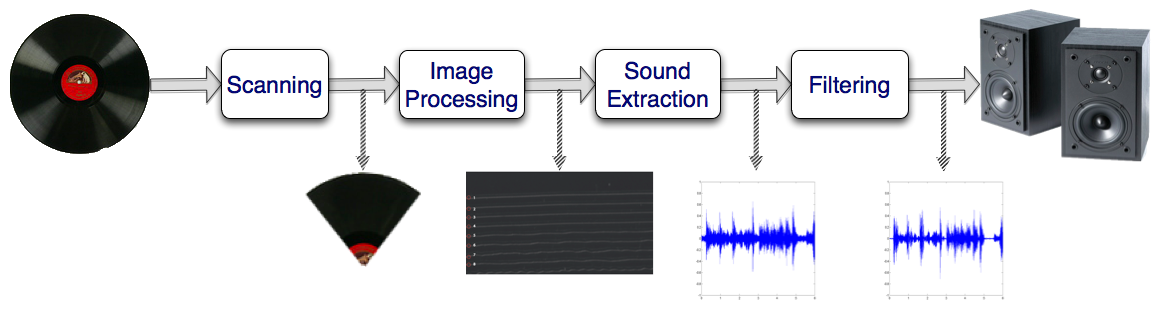
\includegraphics[width=1\textwidth]{immagini/block-scheme.png}
\end{figure}
\end{block}
\end{frame}

\begin{frame}
\frametitle{La realtà di interesse}
\begin{block}{Il processo di scansione: considerazioni preliminari e personali}
Analisi preventiva per capire i problemi da affrontare:
\begin{itemize}
\item Scegliere la risoluzione adatta;
\item Individuare la porzione della scansione con più informazione;
%\item[*] individuare la porzione di disco meglio illuminata (discorsi su ottiche);
\item Come partizionare il disco?
\end{itemize}
\end{block}

\begin{block}{Il processo di scansione: cosa suggerisce la teoria?}
%Studio della letteratura per discriminare tra possibili scelte 
\begin{itemize}
\item Risoluzione 2400 dpi ottici;
\item Non sempre banale la scelta della posizione corretta per la scansione;
\item Scelte per il partizionamento varie (solitamente 4 fette).
\end{itemize}
\end{block}
\end{frame}

\begin{frame}
\frametitle{La realtà di interesse}
\begin{block}{L'elaborazione dell'immagine: cosa suggerisce la teoria}
Individuate tre fasi principali
\begin{itemize}
\item Ricerca del centro;
\item Unwrap dell'immagine;
%\item[*] Passaggio da coordinate cartesiane a polari(la porzione viene spalmata);
\item Crop dell'immagine.
\end{itemize}
\end{block}
\end{frame}

\begin{frame}
\frametitle{La realtà di interesse}
\begin{block}{L'estrazione del suono: considerazioni preliminari}
\'E stato necessario capire molto bene come mappare le variazioni presenti
sul disco, in modo da effettuare una traduzione sensata e fedele.
\end{block}
\begin{block}{L'estrazione del suono: cosa suggerisce la teoria}
\begin{itemize}
\item Ricerca delle tracce;
\item ``Inseguimento'' delle tracce;
\item Concatenzione delle tracce.
\end{itemize}
\end{block}
\end{frame}
